\documentclass[11pt,a4paper]{report}

% Language setting
% Replace `english' with e.g. `spanish' to change the document language
\usepackage[portuges]{babel}
% Set page size and margins
% Replace `letterpaper' with `a4paper' for UK/EU standard size
\usepackage[utf8]{inputenc}
\usepackage{graphicx}
\usepackage{url}
\usepackage{enumerate}
\usepackage{color}
\usepackage{multirow}
\usepackage{array}
\usepackage[pdftex]{hyperref}
\usepackage{listings}
\usepackage{enumitem}
\definecolor{codegreen}{rgb}{0,0.6,0}
\definecolor{codegray}{rgb}{0.5,0.5,0.5}
\definecolor{codepurple}{rgb}{0.58,0,0.82}
\definecolor{backcolour}{rgb}{0.95,0.95,0.92}

\lstdefinestyle{mystyle}{
    backgroundcolor=\color{backcolour},
    commentstyle=\color{magenta},
    keywordstyle=\color{codegreen},
    numberstyle=\tiny\color{codegray},
    stringstyle=\color{codepurple},
    basicstyle=\ttfamily\footnotesize,
    breakatwhitespace=false,
    breaklines=true,
    keepspaces=true,
    numbers=left,
    numbersep=2pt,
    showspaces=false,
    showstringspaces=false,
    showtabs=true
}

\lstset{style=mystyle}

\graphicspath{{../../imagens/TP2/}}

\title{PLC - Trabalho Prático 2\\
    \large Grupo nº14}

\author{
    Simão Pedro Batista Caridade Quintela \\ (A97444) 
    \and David José de Sousa Machado \\ (A91665)
    \and Hugo Filipe de Sá Rocha \\ (A96463)
} %autores do documento

\date{\today} %data

\begin{document}

    \begin{minipage}{0.9\linewidth}
        \centering
        
\includegraphics[width=0.4\textwidth]{um.jpg}\par\vspace{1 cm}
        \href{https://www.uminho.pt/PT}
        {\scshape\LARGE Universidade do Minho} \par
        \vspace{0.6cm}
        \href{https://lcc.di.uminho.pt}
        {\scshape\Large Licenciatura em Ciências da Computação} \par
        \maketitle
        
        
\includegraphics[width=0.3\linewidth]{simao.jpg}
        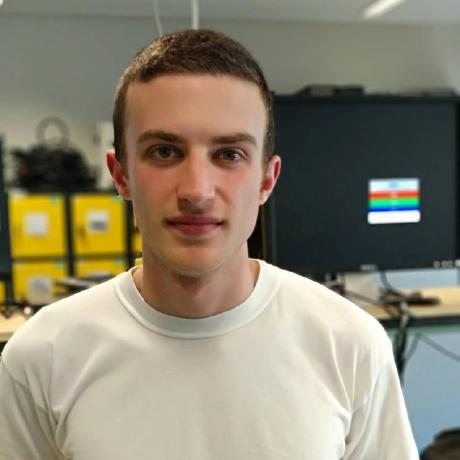
\includegraphics[width=0.3\linewidth]{david.jpg}
        
\includegraphics[width=0.35\linewidth]{hugo.jpg}
    \end{minipage}

    \tableofcontents

    \pagebreak


    \chapter{Introdução}
    \paragraph{}
    No âmbito da disciplina de Processamento de Linguagens e Compiladores foi-nos proposto pelo docente Pedro Rangel Henriques o desenvolvimento de uma Linguagem de Programação Imperativa simples e de um compilador para reconhecer programas escritas nessa linguagem gerando o respetivo código Assembly da Máquina Virtual VM.
    \paragraph{}
    Começamos por tentar encontrar um nome original e atrativo para a nossa linguagem e acabou por nos surgir a ideia de colocar o nome "Python-Like-C" cuja sigla (PLC) coincide com a sigla da Unidade Curricular que integra este trabalho (Processamento de Linguagens e Compiladores).
    \paragraph{}
    Neste documento está apresentada a gramática da nossa linguagem, o código escrito no módulo Lexer e Yacc do Python e ainda, como foi pedido, alguns testes com código escrito na nossa linguagem e o respetivo código Assembly gerado.


    \chapter{Enunciado}
    \paragraph{}
    Pretende-se que comece por definir uma linguagem de programação imperativa simples, a seu gosto.
    Apenas deve ter em consideração que essa linguagem terá de permitir:
    \begin{itemize}
        \item \textit{declarar} variáveis atómicas do tipo \textit{inteiro}, com os quais se podem realizar as habituais operações aritméticas, relacionais e lógicas;
        \item \textit{efetuar} instruções algorítmicas básicas como a \textit{atribuição do valor de expressões numéricas a variáveis};
        \item \textit{ler} do \textit{standard input} e \textit{escrever} no \textit{standard output};
        \item \textit{efetuar} instruções \textit{condicionais} para controlo do fluxo de execução;
        \item \textit{efetuar} instruções cíclicas para controlo do fluxo de execução, permitindo o seu aninhamento.\\
    \underline{Note} que deve implementar pelo menos o ciclo \textbf{while-do}, \textbf{repeat-until} ou \textbf{for-do}.
    \end{itemize}

    Adicionalmente deve ainda suportar, à sua escolha, uma das duas funcionalidades seguintes:
    \begin{itemize}
        \item \textit{declarar e manusear} variáveis estruturadas do tipo \textit{array (a 1 ou 2 dimensões)} de inteiros, em relação aos quais é apenas permitida a operação de indexação (ı́ndice inteiro);
        \item \textit{definir e invocar subprogramas} sem parâmetros mas que possam retornar um resultado do tipo inteiro.
    \end{itemize}


    \chapter{Concepção da Solução}
    Neste capítulo vamos apresentar:
    \begin{itemize}
        \item A sintaxe da linguagem PLC
        \item Os símbolos
        \item O desenho da gramática independente de contexto
        \item Extras
    \end{itemize}
    No nosso trabalho, acabámos por implementar \textit{arrays} unidimensionais e subprogramas sem retorno.


    \section{Sintaxe da Linguagem PLC}
    A sintaxe da linguagem é a seguinte

    \subsection{Declaração de variáveis}
    \begin{lstlisting}[language=Python]
        int x
        int x = 10
        int x[n]
        int x[10] = {1,2,3,4,5,6,7,8,9,10}
    \end{lstlisting}

    \subsection{Operadores de comparação}
    \begin{lstlisting}[language=Python]
        x <= y
        x >= y
        x < y
        x > y
        x == y
    \end{lstlisting}

    \subsection{Operações numéricas}
    \begin{lstlisting}[language=Python]
        x + y
        x - y
        x / y
        x * y
        x % y
        x ++ #(incremento)
        y -- #(decremento)
    \end{lstlisting}

    \subsection{Operadores lógicos}
    \begin{lstlisting}[language=Python]
        x and y
        x or y
        not x
    \end{lstlisting}

    \subsection{Instruções condicionais}
    \begin{lstlisting}[language=Python]
        if (cond):
            ...
        elif (cond):
            ...
        else:
    \end{lstlisting}

    \subsection{Ciclo while}
    \begin{lstlisting}[language=Python]
        while (cond):
            ...
    \end{lstlisting}

    \subsection{Ciclo do-while}
    \begin{lstlisting}[language=Python]
        do:
            ...
        while (cond)
    \end{lstlisting}

    \subsection{Input/Output}
    \begin{lstlisting}[language=Python]
        x = input()
        x = input("Declare the variable with the value: ")
        print("Hello world!")
    \end{lstlisting}

    \subsection{Comentário}
    \begin{lstlisting}[language=Python]
        # isto e um comentario na nossa linguagem
    \end{lstlisting}

    \subsection{Assert}
    A linguagem tem definidos asserts que utilizam as mensagems de erro da Máquina Virtual
    \begin{lstlisting}[language=Python]
        assert (cond)
    \end{lstlisting}

    \section{Símbolos}
    Os simbolos da linguagem são os seguintes:
    \begin{verbatim}
        'INTDec',
        'NUM',
        'ID',
        'ATRIB',
        'EQUIV',
        'LEQ',  # <= - (less or equal)
        'GEQ',  # >= - (greater or equal)
        'GT',   # >  - (greater than)
        'LT',   # <  - (less than)
        'NEQ',  # /= - (not equal -> NEQ -> NECC)
        'LCPARENT',
        'RCPARENT',
        'LSQBRACKET', # left square bracket
        'RSQBRACKET', # right square bracket
        'LCURLBRACKET',
        'RCURLBRACKET',
        'SUM',
        'SUB',
        'DIV',
        'MULT',
        'MOD',
        'INC',
        'DEC',
        'QUOTE', # Símbolo "
        'STRING',
        'NEWLINE',
        'COLON',
        'WS',
        'INDENT',
        'DEDENT',
        'ENDMARKER'
        'IF',
        'ELSE',
        'ASSERT',
        'WHILE',
        'DO',
        'PRINT',
        'INPUT',
        'AND',
        'OR',
        'NOT',
        'DEF',
        'CALL'
    \end{verbatim}

    \section{Desenho da GIC}
    A nossa linguagem é gerada pela seguinte grámatica independente de contexto:
    \begin{verbatim}
      Programa : Decls Corpo
               | Corpo
      Decls    : Decl
               | Decls Decl
      Decl     : INTDec ID
               | INTDec ID ATRIB NUM
               | INTDec ID ATRIB Input 
               | INTDec ID ATRIB INPUT LCBRACKET RCBRACKET
               | INTDec ID LSQBRACKET NUM RSQBRACKET
               | INTDec ID LSQBRACKET NUM RSQBRACKET LSQBRACKET NUM RSQBRACKET
      Corpo    : Proc
               | Corpo Proc
      Newline  : NEWLINE
               | ε
      Proc     : Atrib
               | Print
               | If
               | Cycle
      Print    : NonFormatted
               | Formatted (not implemented)
      NonFormatted : PRINT LCPARENT QUOTE Argument QUOTE RCPARENT
      Formatted : ....
      Argument : String
               | Expr

      If       : IF LCPARENT cond RCPARENT COLON INDENT Corpo Dedent
               | IF LCPARENT cond RCPARENT COLON INDENT Corpo Dedent ELSE COLON INDENT Corpo DEDENT

      Atrib    : ID ATRIB Expr
               | ID ATRIB Input
               | ....

      Cond     : Expr GT Expr 
               | Expr LT Expr
               | Expr GEQ Expr
               | Expr LEQ Expr
               | Expr EQUIV Expr
               | Expr NEQ Expr
               | Cond OR Cond
               | Cond AND Cond
               | NOT Cond

      Expr     : Var                .
               | NUM                .
               | ID INC             . 
               | ID DEC             .
               | ID SUM ATRIB Expr  
               | ID SUB ATRIB Expr
               | Expr SUM Expr      .
               | Expr SUB Expr      .
               | Expr DIV Expr      .
               | Expr MUL Expr      .
               | Expr MOD Expr      .

      Var      : ID
      Input    : INPUT LCPARENT String RCPARENT
      String   : QUOTE STRING QUOTE
               | ε
    \end{verbatim}

    \section{Extras}
    Os extras implementados foram:
    \begin{itemize}
        \item Comentários
        \item Erros
        \item Ordem de operações(simples)
        \item Indentação obrigatória
    \end{itemize}

    \subsection{Comentários}
    \paragraph{}
    Os comentários funcionam através do consumo do padrão sem retornar valor.
    \begin{lstlisting}[language=Python]
        def t_comment(t):
            r'\#.*'
            pass
    \end{lstlisting}

    \subsection{Erros}
    \paragraph{}
    Definimos messagens de erro para ajudar o utilizador a corrigir os erros do seu programa.
    \begin{lstlisting}[language=Python]
        def p_error(p):
            print('Syntax error!\np -> ', p)
            parser.sucesso = False
    \end{lstlisting}

    \subsection{Ordem de operações(simples)}
    \paragraph{}
    Definimos também a precedência dos operadores aritméticos para que o cálculo de uma expressão aritmética seja
     feito de acordo com a precedência habitual dos operadores(não tendo em conta expressões dentro de parêntesis):
    \begin{lstlisting}[language=Python]
        precedence = (
            ("left", "SUM", "SUB"),
            ("left", "MULT", "DIV")
        )
    \end{lstlisting}

    \subsection{Indentação}
    \paragraph{}
    Para implementar a indentação obrigatória inspiramo-nos num dos exemplos da documentação do PLY chamado "GardenSanke".
    O processo de verificação de indentação é feito através de dois filtros que são corridos após o analisador léxico.
    Os tokens utilizados para o processo são o 'COLON', a 'NEWLINE', o 'WS' o 'INDENT' e o 'DEDENT'.
    \paragraph{}
    O primeiro filtro identifica os tokens 'COLON', 'NEWLINE' e 'WS' e utiliza-os para identificar quais os tokens que devem ser indentados e 
    quais os tokens no início das linhas para posteriormente verificar o nível da indentação.
    \paragraph{}
    O segundo filtro calcula as profundidades das indentações a emitir e os tokens 'INDENT' e 'DEDENT' para criar os blocos.
    Nos 'WS' inicializa a profundidade da indentação e retêm o token neste filtro. Nos 'NEWLINE' reinicia profundidade da indentação.
    Nos restantes tokens verifica se a indentação está de acodordo com a respectiva profundidade e emite os seus tokens 'INDENT' e 'DEDENT'
    No final criamos 'DEDENT's que estejam em falta devido à terminação do ficheiro num estado aninhado.



    \chapter{Exemplos de funcionamento}
    --- preencher exemplos -- 


\chapter{Conclusão}
\paragraph{}
Fazendo uma retrospetiva referente ao trabalho prático, entendemos que os todos os objetivos do trabalho prático foram cumpridos. A realização deste trabalho foi particularmente atrativa pois ao desenvolver a nossa própria linguagem de programação somos nós quem decide toda a sua sintaxe e notação e chegar ao fim e perceber que conseguimos desenvolver a base de uma linguagem de programação é satisfatório.
\paragraph{}
A realização deste trabalho prático fez com que ficássemos bem dentro do funcionamento do módulo Lexer e do módulo Yacc, nomeadamente como funciona o reconhecimento de tokens e a implementação da nossa gramática. A geração de código Assembly foi sem dúvida também um ponto positivo deste trabalho pois permitiu-nos entender melhor a linguagem e as suas instruções. 
\paragraph{}
Em suma, entendemos que todos os objetivos foram concluídos e consideramos que este trabalho foi bastante desafiador e uma excelente fonte de conhecimento para desafios futuros. 


\end{document}